\begin{minipage}{0.75\linewidth}
\begin{figure}[h]
    \centering
    \begin{adjustbox}{max width=1.0\linewidth, keepaspectratio}
        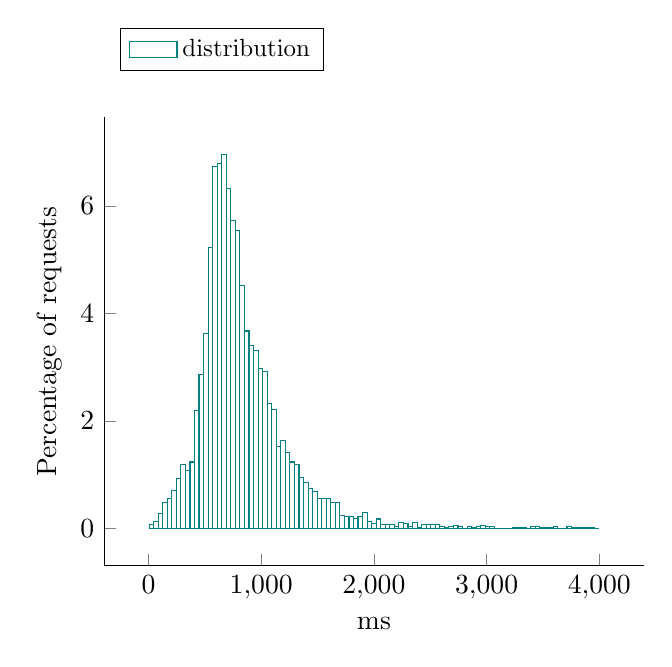
\begin{tikzpicture}
            \begin{axis}[ylabel = Percentage of requests, 
xlabel = ms, 
legend style = {nodes={scale=0.9, transform shape}, at={(0.03,1.2)}, anchor=north west, draw=black, fill=white, align=left, legend columns=3},
area style, mark size = 0pt,
 cycle list name = exotic,
  axis lines* = left]
		\addplot +[ybar interval] coordinates {
			 (5, 0.0625)
			 (45.31, 0.125)
			 (85.62, 0.28125)
			 (125.93, 0.484375)
			 (166.24, 0.546875)
			 (206.55, 0.703125)
			 (246.86, 0.921875)
			 (287.17, 1.1875)
			 (327.48, 1.07812)
			 (367.79, 1.23438)
			 (408.1, 2.1875)
			 (448.41, 2.85938)
			 (488.72, 3.625)
			 (529.03, 5.21875)
			 (569.34, 6.73437)
			 (609.65, 6.78125)
			 (649.96, 6.95312)
			 (690.27, 6.32812)
			 (730.58, 5.73438)
			 (770.89, 5.54688)
			 (811.2, 4.51562)
			 (851.51, 3.67188)
			 (891.82, 3.40625)
			 (932.13, 3.3125)
			 (972.44, 2.96875)
			 (1012.75, 2.92188)
			 (1053.06, 2.32812)
			 (1093.37, 2.20312)
			 (1133.68, 1.51562)
			 (1173.99, 1.64062)
			 (1214.3, 1.40625)
			 (1254.61, 1.23438)
			 (1294.92, 1.1875)
			 (1335.23, 0.9375)
			 (1375.54, 0.859375)
			 (1415.85, 0.734375)
			 (1456.16, 0.6875)
			 (1496.47, 0.546875)
			 (1536.78, 0.546875)
			 (1577.09, 0.546875)
			 (1617.4, 0.484375)
			 (1657.71, 0.484375)
			 (1698.02, 0.234375)
			 (1738.33, 0.21875)
			 (1778.64, 0.21875)
			 (1818.95, 0.1875)
			 (1859.26, 0.21875)
			 (1899.57, 0.296875)
			 (1939.88, 0.125)
			 (1980.19, 0.09375)
			 (2020.5, 0.171875)
			 (2060.81, 0.078125)
			 (2101.12, 0.0625)
			 (2141.43, 0.0625)
			 (2181.74, 0.03125)
			 (2222.05, 0.109375)
			 (2262.36, 0.09375)
			 (2302.67, 0.03125)
			 (2342.98, 0.109375)
			 (2383.29, 0.015625)
			 (2423.6, 0.0625)
			 (2463.91, 0.0625)
			 (2504.22, 0.0625)
			 (2544.53, 0.0625)
			 (2584.84, 0.03125)
			 (2625.15, 0.015625)
			 (2665.46, 0.03125)
			 (2705.77, 0.046875)
			 (2746.08, 0.03125)
			 (2786.39, 0)
			 (2826.7, 0.03125)
			 (2867.01, 0.015625)
			 (2907.32, 0.03125)
			 (2947.63, 0.046875)
			 (2987.94, 0.03125)
			 (3028.25, 0.03125)
			 (3068.56, 0)
			 (3108.87, 0)
			 (3149.18, 0)
			 (3189.49, 0)
			 (3229.8, 0.015625)
			 (3270.11, 0.015625)
			 (3310.42, 0.015625)
			 (3350.73, 0)
			 (3391.04, 0.03125)
			 (3431.35, 0.03125)
			 (3471.66, 0.015625)
			 (3511.97, 0.015625)
			 (3552.28, 0.015625)
			 (3592.59, 0.03125)
			 (3632.9, 0)
			 (3673.21, 0)
			 (3713.52, 0.03125)
			 (3753.83, 0.015625)
			 (3794.14, 0.015625)
			 (3834.45, 0.015625)
			 (3874.76, 0.015625)
			 (3915.07, 0.015625)
			 (3955.38, 0)
			 (3995.69, 0)
		};
\addlegendentry{distribution};
           \end{axis}
      \end{tikzpicture}
  \end{adjustbox}
  \caption{Response time distribution - req = ReadTimeline-2}
\end{figure}
\end{minipage}\hfill\begin{minipage}{0.18\linewidth}
\begin{table}[h]
\begin{tabular}{|cc|}
\hline
\textbf{} & \textbf{ms}\\ \hline
 \Xhline{0.005\arrayrulewidth}
min & 5\\
 \Xhline{0.005\arrayrulewidth}
max & 4036\\
 \Xhline{0.005\arrayrulewidth}
mean & 836\\
 \Xhline{0.005\arrayrulewidth}
std & 405\\
\hline
\hline
 \Xhline{0.005\arrayrulewidth}
25th & 596\\
 \Xhline{0.005\arrayrulewidth}
50th & 747\\
 \Xhline{0.005\arrayrulewidth}
75th & 994\\
 \Xhline{0.005\arrayrulewidth}
80th & 1065\\
 \Xhline{0.005\arrayrulewidth}
85th & 1161\\
 \Xhline{0.005\arrayrulewidth}
90th & 1303\\
 \Xhline{0.005\arrayrulewidth}
95th & 1553\\
 \Xhline{0.005\arrayrulewidth}
99th & 2347\\
\hline
\end{tabular}
\caption{Response time}
\end{table}
\end{minipage}\hfill